\documentclass{article}
\usepackage{tikz}

\begin{document}

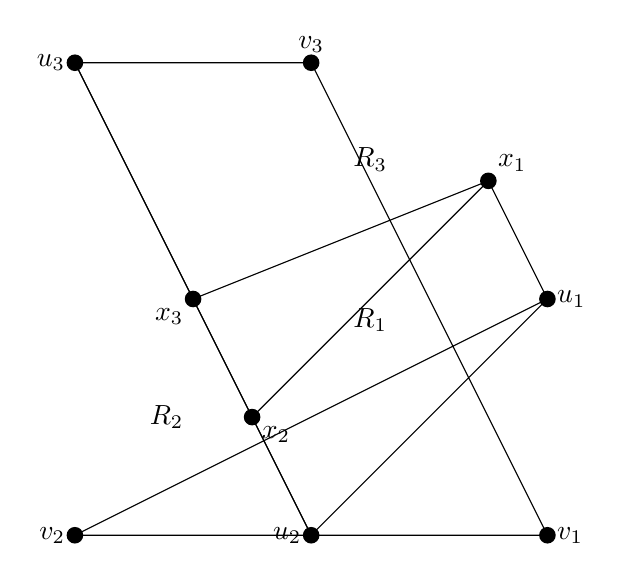
\begin{tikzpicture}[scale=1.5]
    % Define coordinates for the vertices
    \coordinate (u1) at (4,0);
    \coordinate (u2) at (2,-2);
    \coordinate (u3) at (0,2);
    \coordinate (v1) at (4,-2);
    \coordinate (v2) at (0,-2);
    \coordinate (v3) at (2,2);
    \coordinate (x1) at (3.5,1);
    \coordinate (x2) at (1.5,-1);
    \coordinate (x3) at (1,0);

    % Draw the vertices
    \foreach \point in {u1,u2,u3,v1,v2,v3,x1,x2,x3} {
        \fill (\point) circle (2pt);
    }

    % Draw the edges
    \draw (u1) -- (u2) -- (u3) -- (v3) -- (v1) -- (v2) -- cycle;
    \draw (u1) -- (x1);
    \draw (u2) -- (x2);
    \draw (u3) -- (x3);
    \draw (x1) -- (x2);
    \draw (x1) -- (x3);
    \draw (x2) -- (x3);

    % Label the vertices
    \node at (u1) [right] {$u_1$};
    \node at (u2) [left] {$u_2$};
    \node at (u3) [left] {$u_3$};
    \node at (v1) [right] {$v_1$};
    \node at (v2) [left] {$v_2$};
    \node at (v3) [above] {$v_3$};
    \node at (x1) [above right] {$x_1$};
    \node at (x2) [below right] {$x_2$};
    \node at (x3) [below left] {$x_3$};

    % Label the regions
    \node at (2.5,0) [below] {$R_1$};
    \node at (1,-1) [left] {$R_2$};
    \node at (2.5,1) [above] {$R_3$};
\end{tikzpicture}

\bigskip

$x_3 \in X_3$ is the middle vertex of some $P_5(u_1,u_2)$.

\end{document}